\section{Multilayer Perceptron Trained on Synthetic Objects}
\label{sec:simple_mlp}

In our first experiment, we encode the categorical stimulus information of our
synthetic objects as abstract patterns, representing the shape, color and
texture features each as independent 20-bit vectors. The overall stimulus thus
has 60 bits. The categories of each feature are assigned their bit-vector representations
randomly at the beginning of the experiment. We train a multilayer perceptron (MLP)
with one hidden layer of 30 ReLU units to classify the shape of the presented
stimulus. The number of units in the softmax layer varies with the
\textit{\# categories} dataset parameter. To mimick the control group of
\cite{Smith2002}, we initialized our MLP model randomly and evaluated
second-order generalization results prior to training. The model selected by
shape X\%, color X\% and texture X\% We then trained our model with various
dataset sizes. Results for each the first- and second-order generalizations,
averaged over 10 training runs, are shown in Fig. \ref{fig:mlp_gen_results}.
TODO: discuss results.

To analyze the parametric dependency of network biases on the presented
stimuli, we perform a series of tests using a network trained with 50 categories
and 15 exemplars. For the first test, we probe the shape bias of our MLP by
varying the shape distance between two presented stimuli and recording the resulting
network similarity score at each input pair, using cosine similarity at the
hidden layer. Distance in shape space is quantified as the fraction of bits that
differ along the 20-bit space denoted to shape. Similar tests are also performed
for the color and texture features. Results are shown in Fig.
\ref{fig:mlp_parametric}. TODO: discuss results.

\begin{figure}[h!]
    \begin{center}
        \begin{subfigure}[b]{0.235\textwidth}
            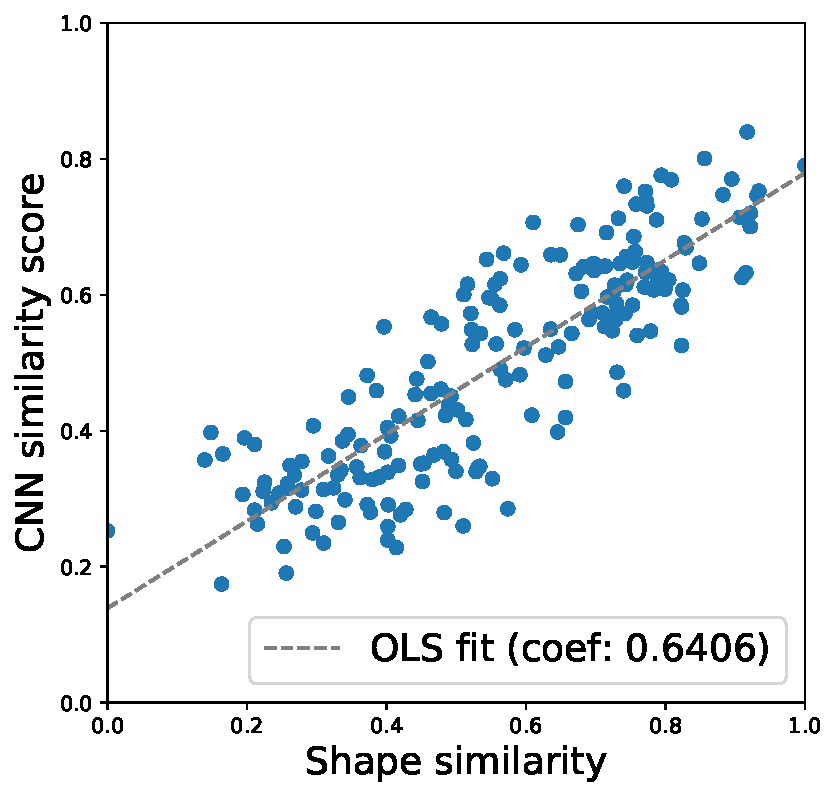
\includegraphics[width=\linewidth]
            {figures/vgg_shape_parametric_others_constant.pdf}
            \caption{Shape}
        \end{subfigure}
        \begin{subfigure}[b]{0.235\textwidth}
            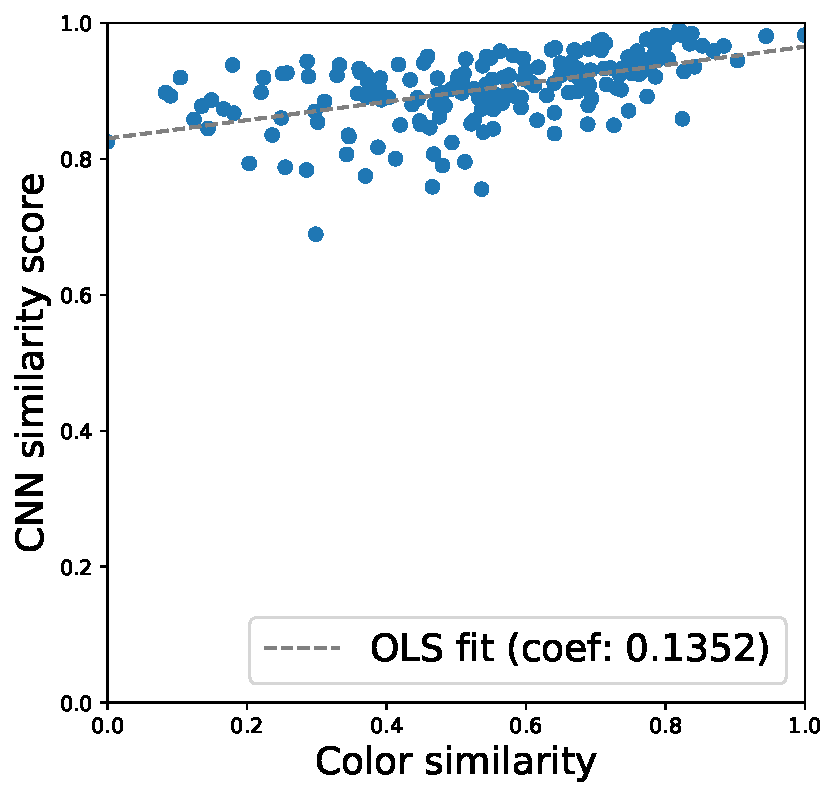
\includegraphics[width=\linewidth]
            {figures/vgg_color_parametric_others_constant.pdf}
            \caption{Color}
        \end{subfigure}
    \end{center}
    \caption{MLP parametric shape and color biases. TODO: put correct result
    plots here.}
    \label{fig:mlp_parametric}
\end{figure}